\documentclass{elsarticle}

\usepackage{amsmath}
\usepackage{amssymb}
\usepackage{graphicx}
\usepackage{url}
\usepackage{boxedminipage}

\setcounter{tocdepth}{3}
\def\keywordname{{\textbf{Keyword:}}}
\newcommand{\keywords}[1]{\par\addvspace\baselineskip
\noindent\keywordname\enspace\ignorespaces#1}

\journal{Journal of Web Semantics}

\begin{document}

\begin{frontmatter}

\title{An Ontology-driven Architecture for Extensible Scientific Data Management Systems}

\author{Yuan-Fang Li\corref{cor1}}
\ead{uqyli4@uq.edu.au}
\author{Gavin Kennedy}
\ead{g.kennedy1@uq.edu.au}
\author{Faith Davies}
\ead{f.davies@uq.edu.au}
\author{Jane Hunter}
\ead{j.hunter1@uq.edu.au}

\cortext[cor1]{Author for correspondence}

\address{School of ITEE, The University of Queensland\\
GP South, Staff House Road, St Lucia 4072, Australia}

\begin{abstract}
Data management has become a critical challenge faced by a wide
array of scientific disciplines in which the provision of sound data
management is pivotal to the success and impact of research
projects. The huge and rapidly growing amounts of data to be managed
and the fact that the \emph{models} of data evolve over time
contribute to making data management an increasingly complex
undertaking that warrants a rethinking of its design. We believe
that a number of intrinsic characteristics of Semantic Web ontology
languages OWL and RDFS, such as semantic rigor and the extensible
nature, make them an ideal conceptual platform on which effective
data management systems can be developed. In this paper, we present
our efforts in designing an open and extensible architecture with an
ontology at its core. In this architecture, the behaviors of domain
concepts and objects are captured entirely by ontological entities,
around which all data management tasks are carried out. Moreover,
the open and semantic nature of ontology languages also makes such
systems amenable to greater data reuse and interoperability. To the
best of our knowledge, this is the first proposal of an
ontology-driven architecture for extensible data management systems.
An ideal domain for applying these principles is phenomics, the
systematic study of phenotypes of organisms. Phenomics research
generates high volumes of heterogeneous data and makes use of
emerging imaging and measurement technologies and processes, thus
making it an ideal testbed for data management systems. In this
context, we describe the development of PODD, a data management
system for phenomics research, as a step towards validating the
practicality of the ontology-driven architecture.
\end{abstract}

\begin{keyword}
Ontology-driven architecture \sep OWL \sep data management systems \sep PODD
\end{keyword}

\end{frontmatter}

\section{Introduction and Background}\label{sec:intro}
Data management is the practice of managing (digital) data
and resources, encompassing a wide range of
activities including acquisition, storage, retrieval, discovery,
access control, publication, integration, curation and archival.
For many data-intensive scientific disciplines such as life sciences and
bioinformatics, sound data management informs and enables
research and it has become an indispensable component~\cite{1107503}.

The need for effective data management is, in a large part, due to
the fact that huge amounts of digital data are being generated by
modern instruments.
% some stats/citations?
Furthermore, the fast evolution of technologies/processes and
discovery of new scientific knowledge require flexibility in
handling dynamic data and models in data management systems.

Database systems have traditionally been used successfully
to manage research data~\cite{brm2007}. Database schemas are
used as domain models to capture the attributes and relationships
of domain concepts. One implication of the above approach is
that domain models need to stay relatively stable as database
extension or migration is often an error-prone and laborious task
in practice. Hence, we believe that this approach is not suitable
for domains where data and model evolution is the
norm rather than the exception.

Semantic Web ontology languages such as RDF
Schema~\cite{rdfschema04} and OWL~\cite{hoph03a} possess
expressive, rigorously-defined
semantics and non-ambiguous syntaxes. Moreover, they have been
designed to be open and extensible to support knowledge and data
exchange on the Web scale~\cite{linkeddata,aue07dbpedia}.
These intrinsic characteristics make them an ideal conceptual
platform on which a flexible data management system that supports
dynamic data and models can be built.

Ontology language OWL has been widely used in a number of domains,
notably in life sciences and
biotechnology~\cite{journals/bib/RuttenbergRSM09,citeulike:1882392,citeulike:212874}
as a modeling language for its expressivity and extensibility. There
is also growing tool support for tasks such as reasoning, querying
and visualization, making it a viable option for the modeling and
representation of scientific domain concepts.

Moreover, with the rapid progression of Semantic Web-based
data integration through the community-driven Linked Data
project~\cite{citeulike:5008761},
it is advantageous for data management systems to support
Semantic Web languages and standards natively to benefit
from the fast-increasing, integrated open datasets.

In this paper, we present our work in designing
a domain-independent, ontology-driven architecture for scientific
data management systems. In our architecture, we support data and model
dynamics through ontology-based domain modeling. In this architecture,
the ontology is at the core of the system where the behaviors of
abstract domain concepts and concrete domain objects are entirely
defined with ontological vocabularies. Logical structure of
data is therefore maintained and enforced via ontological
definitions and reasoning and not via database schemas and associated
constraints.

We also describe the modeling of the base ontology in
this architecture and show how the domain can be
conceptualized in an ontology in an extensible and
flexible way.

Based on such a design, we have developed the Phenomics Ontology
Driven Data (PODD) data management system~\cite{podd_icadl} that
supports the effective management of large-scale, evolving data for
phenomics research. An example of concept change is the concept
\emph{GrowthCondition} in phenomics, which captures the
environmental conditions in which an organism grows. For different
disciplines and projects, it can be specialized to
\emph{CabinetCondition} to capture conditions in controlled
environments and \emph{FieldCondition} to capture conditions in the
field.

The ontology-based domain model is at the core of PODD as it drives
the creation, storage, validation, query and search of data and
metadata. In contrast to traditional data management systems that
use database schemas as the underlying model, the employment of OWL
ontologies as the domain model makes PODD highly extensible.

In biology, an organism's phenotype is its observable or
quantifiable trait, such as the height of a plant or the size of a
leaf, as a consequence of its genetic makeup combined with its
developmental stage, environment and disease conditions. Phenomics
is the systematic and comprehensive study of an organism's phenotype
and is determined through a combination of high-throughput and
high-resolution imaging- and measurement-based analysis platforms.
Phenomics research, together with genomics research, represents a
holistic and promising new approach to biological
study~\cite{dhoule09,Sauer200458,nevo01,plant_furbank}.

Unlike genomics, phenomics research emphasizes the study of
physical, observable traits of organisms. Like genomics, vast
amounts of data are produced by imaging and measurement platforms
and analysis tools. The effective storage, management, analysis and
discovery of these data is a challenging problem. Specifically,
there are three key challenges for data management in phenomics
research.
\begin{itemize}
\item The ability to provide a data management service that can
manage large quantities of heterogeneous data in multiple formats
(text, image, video) and not be constrained to a finite set of
imaging and measurement platforms and data formats.

\item The ability to support metadata-related services to
provide context and structure for data within the data management
service to facilitate effective search, query and dissemination.

\item The ability to accommodate evolving and emerging technologies
and processes as phenomics is still a rapidly developing field of
research.
\end{itemize}

PODD has been developed to meet the above challenges facing
the Australian phenomics research community by providing
efficient and flexible repository functionalities for large-scale
phenomics data, and providing a mechanism
for maintaining structured and precise \emph{metadata} around the
raw data so that they can be stored, distributed and published
in a reusable fashion. We would like to emphasize that although
the PODD system is geared
towards phenomics research, the ontology-driven architecture
we propose in this system is actually domain-independent and can be
applied in any scientific discipline where research output can
be conceptually organized in a structured manner.
%We will describe the PODD system and show how the ontology-based
%architecture is realized through leveraging mature open-source
%technologies. In the implementation of the PODD system, we have
%made some careful design decisions, which will be documented
%in the paper as well.

%In this paper, we present our work in addressing the above
%challenges and highlight the OWL-based modeling approach we take.
The rest of the paper is organized as follows. In
Section~\ref{sec:overview} we present related work and give a
brief overview of the motivation and goals of the PODD
project. Section~\ref{sec:design} presents in detail the
ontology-based architecture for data management systems.
In Section~\ref{sec:ont}, in a bioinformatics setting,
we discuss the PODD domain ontology in more detail and
show how the ontology-based modeling
approach is used in the life cycle of domain objects.
In Section~\ref{sec:podd}, we describe the implementation
of the PODD data management system. Finally,
Section~\ref{sec:conclusion} concludes the paper and identifies
future directions.

\section{Related Work, Motivation \& Goals}\label{sec:overview}
Over the years attempts have been made to develop content repository
systems and architectures to meet institutional and personal
data management needs. In this section, we introduce a number of
such systems and architectures. With a survey of related work,
we present the motivation behind the ontology-driven architecture
and the goals we wish to achieve with the PODD data management system.

\subsection{Data and Resource Management Systems}
A number of open-source content repository specifications and
software systems have been developed.

Fedora Commons\footnote{\url{http://www.fedora-commons.org/}} is an open-source
digital resource management system based on the principles of modularity,
interoperability and extensibility. In Fedora Commons, abstract concepts are defined
as \emph{models}, on which inter-relationships and behaviors
can be further defined. Data in Fedora Commons repositories are
organized into \emph{objects}, which have \emph{datastreams} that stores
either metadata or data. Fedora Commons makes heavy use of Semantic Web
technologies through the use of common RDF vocabularies and the integration
with the Mulgara triple store\footnote{\url{http://www.mulgara.org/}},
which can be used for metadata storage and query through SPARQL.
Fedora Commons has been used as a backend to implement document
management systems, digital libraries and institutional repositories.

Apache Jackrabbit\footnote{\url{http://jackrabbit.apache.org/}} is an
open-source implementation of the Content Repository for Java Technology
(JCR) API\footnote{\url{http://jcp.org/en/jsr/detail?id=283}}. In JCR,
data is stored in a tree of \emph{nodes}, which can hold \emph{properties}
of arbitrary values, which is conceptually similar to Fedora Commons.
Types can be defined on nodes to place certain restrictions on them.

Fedora Commons and JCR both support fairly basic mechanisms for
defining object relationships. Hence, they are usually used as the
underlying repository solution on which complex data and document
management systems are built. These systems include Biodiversity
Heritage Library\footnote{\url{http://www.biodiversitylibrary.org/}}
and Fez\footnote{\url{http://fez.library.uq.edu.au/}}, among others.
As stated previously, these systems use database schemas as their
domain models.

Data management systems have also been developed to support a number
of scientific disciplines including high-energy physics, bioinformatics
and Earth observation.

Bioinformatics Resource Manager (BRM)~\cite{brm2007} is one example of
client-server style data management software for bioinformatics
research. The client software is installed on users' computers to access
(microarray and proteomic) resources stored on BRM server in a
PostgreSQL relational database.
The BRM server supports data acquisition from external sources such as
NCBI~\cite{DBLP:journals/nar/WheelerBBBCCCDEFGHKKKLMMOPSSSSSSSSTTWY06}
and UniProt~\cite{AmosBairoch01012005}. It also supports annotation
using public datasets and connectivity to analytics tools. Data in
BRM is stored under the \emph{Project} concept and is mostly flat, i.e.,
it does not support hierarchical domain concepts such as investigation
and publication.

Besides data management systems, grid-based middleware
systems have also been developed to provide distributed
storage solutions. Such systems include the Storage
Resource Broker (SRB)~\cite{783165} and the CERN Data Grid~\cite{652836}
and other systems that make use of Globus\footnote{\url{http://www.globus.org/}}
middleware. These systems store data in a distributed environment
and usually support authentication, replication, redundancy, etc.
However, they are mostly only concerned about data storage and
replication and hence do not provide full-fledged data management
capabilities. Interested readers can see~\cite{565296}
for a detailed survey of grid resource management systems.

\subsection{Domain Modeling in Scientific Research}
A number of specifications and ontologies have been proposed to
model scientific research activities. In 2004, Council for the
Central Laboratory of the Research Councils (CCLRC) of UK developed
a CCLRC Scientific Metadata Model~\cite{Spallation_metadatamodel}
that models scientific activities in free text. An OWL ontology,
EXPO, was developed~\cite{citeulike:3735746} to capture metadata
about scientific experiments. EXPO was developed in a top-down
approach by extending concepts in the Suggested Upper Merged
Ontology (SUMO)\footnote{\url{http://www.ontologyportal.org/}}.
Although very comprehensive, these models are very verbose and not
very suitable as a model for developing data management systems.

In biological and particularly 'omics research,
a large number of databases have been
developed to host a variety of information such as genes
(Ensembl\footnote{\url{http://www.ensembl.org/}}), proteins
(UniProt\footnote{\url{http://www.uniprot.org/}}), scientific
publications (PubMed\footnote{\url{http://www.ncbi.nlm.nih.gov/pubmed/}}) and
microarray data (GEO\footnote{\url{http://www.ncbi.nlm.nih.gov/geo/}}).
These databases are generally characterized by the fact that they
specialize in a particular kind of data (protein sequences,
publications, etc.) and their conceptual domain models,
such as gene and gene products~\cite{citeulike:212874}
and microarray experiments~\cite{citeulike:151946},
are well understood.

For a scientific data management system to be effective, models of
domain concepts need to be integrated with models of scientific
activities and workflows. However, models of biological and clinical
investigations are less well understood.

The Ontology for Biomedical Investigations
(OBI)\footnote{\url{http://purl.obolibrary.org/obo/obi}} is an
ongoing effort of developing an integrative ontology for biological
and clinical investigations. It takes a top-down approach by reusing
high-level, abstract concepts from other ontologies. It includes
2,600+ OWL~\cite{hoph03a} classes and 10,000+ axioms (in the import
closure of the OBI ontology). Although OBI is very comprehensive,
its size and complexity makes reasoning and querying of OBI-based
ontologies and RDF graphs computationally expensive and time
consuming, making it impractical as a domain model for a data
management system where such reasoning may need to be performed
repeatedly.

Functional Genomics Experiment Model (FuGe)~\cite{citeulike:1756058}
is an extensible modeling framework for high-throughput functional
genomics experiments, aiming at increasing the consistency and
efficiency of experimental data modeling for the molecular biology
research community. Centered around the concept of experiments, it
encompasses domain concepts such as protocols, samples and data.
FuGe is developed using UML from which XML Schemas and database
definitions are derived. The FuGe model covers not only
biology-specific information such as molecules, data and
investigation, it also defines commonly used concepts such as audit,
reference and measurement. Extensions in FuGe are defined using
inheritance of UML classes.

We feel that the extensibility we require is not met by FuGe as any
addition of new concepts would require the development of new
database schemas and code. Moreover, the concrete objects reside in
relational databases, making subsequent integration and
dissemination more difficult.

\subsection{The PODD Data Management System -- Motivation \& Goals}
Phenomics is a fast-growing, data-intensive discipline
with new technologies and processes rapidly emerging
and evolving. As a result, its domain model and data
management systems must also be able to evolve to handle
the complexity, change and scale.

The PODD system is being developed on behalf of two major phenomics
initiatives: the Australian Plant Phenomics Facility (APPF),
specializing in phenotyping crop and model plant species; and the
Australian Phenomics Network (APN), specializing in the
phenotyping of mouse models. Both facilities have common
requirements to gather and annotate data from both high- and
low-throughput phenotyping devices. The scale of measurement can be
from the micro or cellular level, through the level of a single
organism, and up to (in the case of the APPF) the macro or field
level. Imaging, measurement and analysis of organisms on such a large
scale will produce an enormous amount of data.
For example, it has been estimated that more than
60 TB of image data will be generated by APPF research centers
every year, which need to be managed effectively.

Phenomics research makes use of a large variety of imaging and
measurement platforms. For example, in mouse histopathology and
organ pathology research, the Zeiss ``Mirax Scan'' scanner is used
to scan microscope slides. In clinical pathology, a Flow Cytometer
is used to capture laser diffraction images of blood samples. In
plant research, the Lemnatec Scanalyzer is used to capture RGB
images of plants in growth cabinets. The Fluorogroscan system is
used in quenching analysis: the partitioning of light energy used in
photosynthesis on model plants such as Arabidopsis. Other devices,
such as Infrared Thermography Camera to capture leaf temperature and
SPAD Meter to measure the chlorophyll content of plant leaves, are
also used. New devices and instruments will also be used when they
become available. Moreover, existing instruments may be upgraded so
that they can capture more information. The PODD domain model needs
to be flexible to accommodate these changes.

Because an organism's phenotype is often the product of the organism's
genetic makeup, combined with its development stage, disease conditions
and its environment, any measurement made against an organism needs to
be recorded in the context of these other \emph{metadata}. Consequently
the opportunity exists to create a repository to record the data, its
contextual data (metadata) and data classifiers in the form of
ontological or structured vocabulary terms. The structured nature of
this repository would support manual and autonomous data discovery as
well as provide the infrastructure for data based collaborations with
domestic and international research institutions. Currently there are
no such integrated systems available to the two facilities. The
National eResearch Architecture Taskforce (NeAT) Australia initiated
the PODD project to fill this gap. In PODD, we have engaged in the
design and development of the Phenomics Ontology Driven Data (PODD)
repository. The goals of PODD are to capture, manage, annotate and
distribute the data generated by mouse and plant phenomics research
activities. It supports both Australian and international biological
research communities by providing repository and data publication
services.

\section{The Architecture of the Ontology-driven Data Management System}\label{sec:design}

\subsection{Requirements of Data Management Systems}
For any scientific data management systems, a number of requirements
need to be satisfied.

\begin{description}
\item [Data storage and management]
Research activities in data-intensive disciplines such as
'omics often generate huge amounts of data. The ability to efficiently acquire, store and
manage large volumes of data is essential.

\item [Data contextualization]
Sufficient contextual information needs to be maintained for
more effective organization, understanding and discovery of raw data.
Contextual information includes both conceptual
domain models, such as how research activities are organized
and carried out; and metadata such as provenance information.

\item [Data security]
There are many dimensions to data security, including access control,
versioning and backup. An effective data management system needs to
ensure data security through the use of authentication and
authorization and sound versioning and backup solutions.

\item [Data identification and longevity] In order to support the
dissemination of scientific findings, data in the repository needs
to be publicly accessible after being published. Hence, a persistent
and unique naming scheme is required. Moreover, valuable scientific
data also need to be stored in perpetuity.

\item [Data reuse and integration]
Contextual information helps to make sense of raw data.
Moreover, it also needs to be made discoverable,
through means such as full-text search, faceted browsing
and complex query answering, to allow raw data to be integrated and reused.

\item [Model extensibility]
A data management system may need to manage a wide
variety of data, which may be generated by different software
and captured by different platforms. An expressive and extensible
domain model is therefore essential to cater for modification,
addition and deletion of domain concepts. The data management
system also needs to be designed to minimize service disruption
when such a model change occurs.

\end{description}

\subsection{The Ontology-driven Architecture For Data Management Systems}
The most distinguishing characteristic of the ontology-driven architecture
is the central role ontologies play. In this architecture,
raw data are not stored in a flat structure but are attached in
domain objects organized in a logical, hierarchical
system, defined according to the domain model that
represents the structure of research activities.

Current document management systems such as
Fez\footnote{\url{http://fez.library.uq.edu.au/}} typically have a
relatively static domain model and hardwire it as relational schemas
and foreign-key constraints in a custom relational database
independent from the underlying repository system. Consequently, the
information pertinent to the model of each concrete object is stored
in this custom database as well. As stated in the previous section,
this approach is unsuitable for dynamic environments where
conceptual changes are common.

To effectively support a dynamic conceptual framework, the domain
model in the proposed architecture is defined using OWL ontologies,
in which: OWL classes represent domain concepts; OWL properties
define concept attributes and their relationships; OWL restrictions
specify constraints on concepts and finally; OWL individuals define
concrete domain objects where attributes and relationships are
defined using OWL assertions. Raw data files are attached to
concrete domain objects.

Such a conceptual architecture alleviates the problem of imposing hard
relational constraints in a database which is difficult to extend/change.
It is worth noting that referential integrity is not sacrificed in achieving
flexibility: ontological reasoning involving relevant concepts and objects
are performed before object modification to ensure that all constraints
are satisfied.

Another drawback of existing systems is that there can be only one
domain model. When a concept needs to be updated, all the existing
objects need to be updated accordingly, which may be undesirable,
inappropriate and time-consuming. This is, unfortunately, unavoidable
as long as the domain model is defined using database schemas. In our
proposed architecture,
as concept and object definitions are stored in the repository,
such changes can be versioned so that existing instance objects
can remain legitimate when integrity validation is performed as they
can still refer to the previous conceptual definitions.

Similarly, the data and metadata (including ontological definitions)
of each object can be modified, and the modifications should be
versioned so that they can be rolled back.

The major differences between the ontology-driven architecture
and that of current systems can be summarized in Table~\ref{tab:diff} below.

\begin{table}[htdp]
\footnotesize
\centering
\caption{Summary of major conceptual differences between the ontology-driven
architecture and current systems.}\label{tab:diff}
\begin{center}
\begin{tabular}{p{50pt}|p{120pt}|p{120pt}}
\textbf{Aspect}  & \textbf{PODD} & \textbf{Current systems}\\
\hline
Domain modeling & OWL Ontologies & Database schemas\\
\hline
Model organization & In repository, using OWL classes, properties \& individuals & In custom databases, hardwired\\
\hline
Object organization & Ontological definition an integral part, stored in the repository & Stored in databases\\
\hline
Model change & Creates new version of OWL definitions, old objects unaffected & Database \& schema migration, old objects need to be updated\\
\hline
Object change & Creates new version of OWL definitions & Table updates\\
\hline
Referential integrity & OWL reasoning & Database integrity check
\end{tabular}
\end{center}
\end{table}

In developing the ontology-driven architecture,
the following design decisions have been made to balance expressivity,
flexibility and conceptual clarity.

\begin{itemize}
\item There is a top-level domain concept, called \emph{Project}
\footnote{The choice of concept names in the domain ontology is actually
irrelevant to the proposed architecture. Names such as \emph{Project}
and others are chosen as they are general and representative enough.},
under which other concepts (such as \emph{Investigation} and
\emph{Material}) reside in a hierarchical manner.

\item Access control (authorization) is defined on the \emph{Project}
level but not on an individual object level, i.e., a given user will have
the same access rights for all objects within a given project.

\item Within a \emph{Project} hierarchy, objects are in
a parent-child relationship in a tree structure such that
each child can only have one parent. This ensures that
access rights are properly propagated from parent to
child and there is no chance of confusion.

\item Additionally, inter-object, many-to-many reference
relationships can be defined to enhance flexibility of the
architecture as it allows arbitrary links between objects
to be established.

\item Objects cannot be shared across \emph{Projects}. Instead,
objects must be copied from one project and pasted into another one.
Such a rule simplifies object management with the elimination of
possible side-effects caused by sharing object between projects.

\item There should be no interference between different
versions of a given concept and between objects that are instances of
different concept versions.
\end{itemize}

\begin{figure}[htb]
\centering
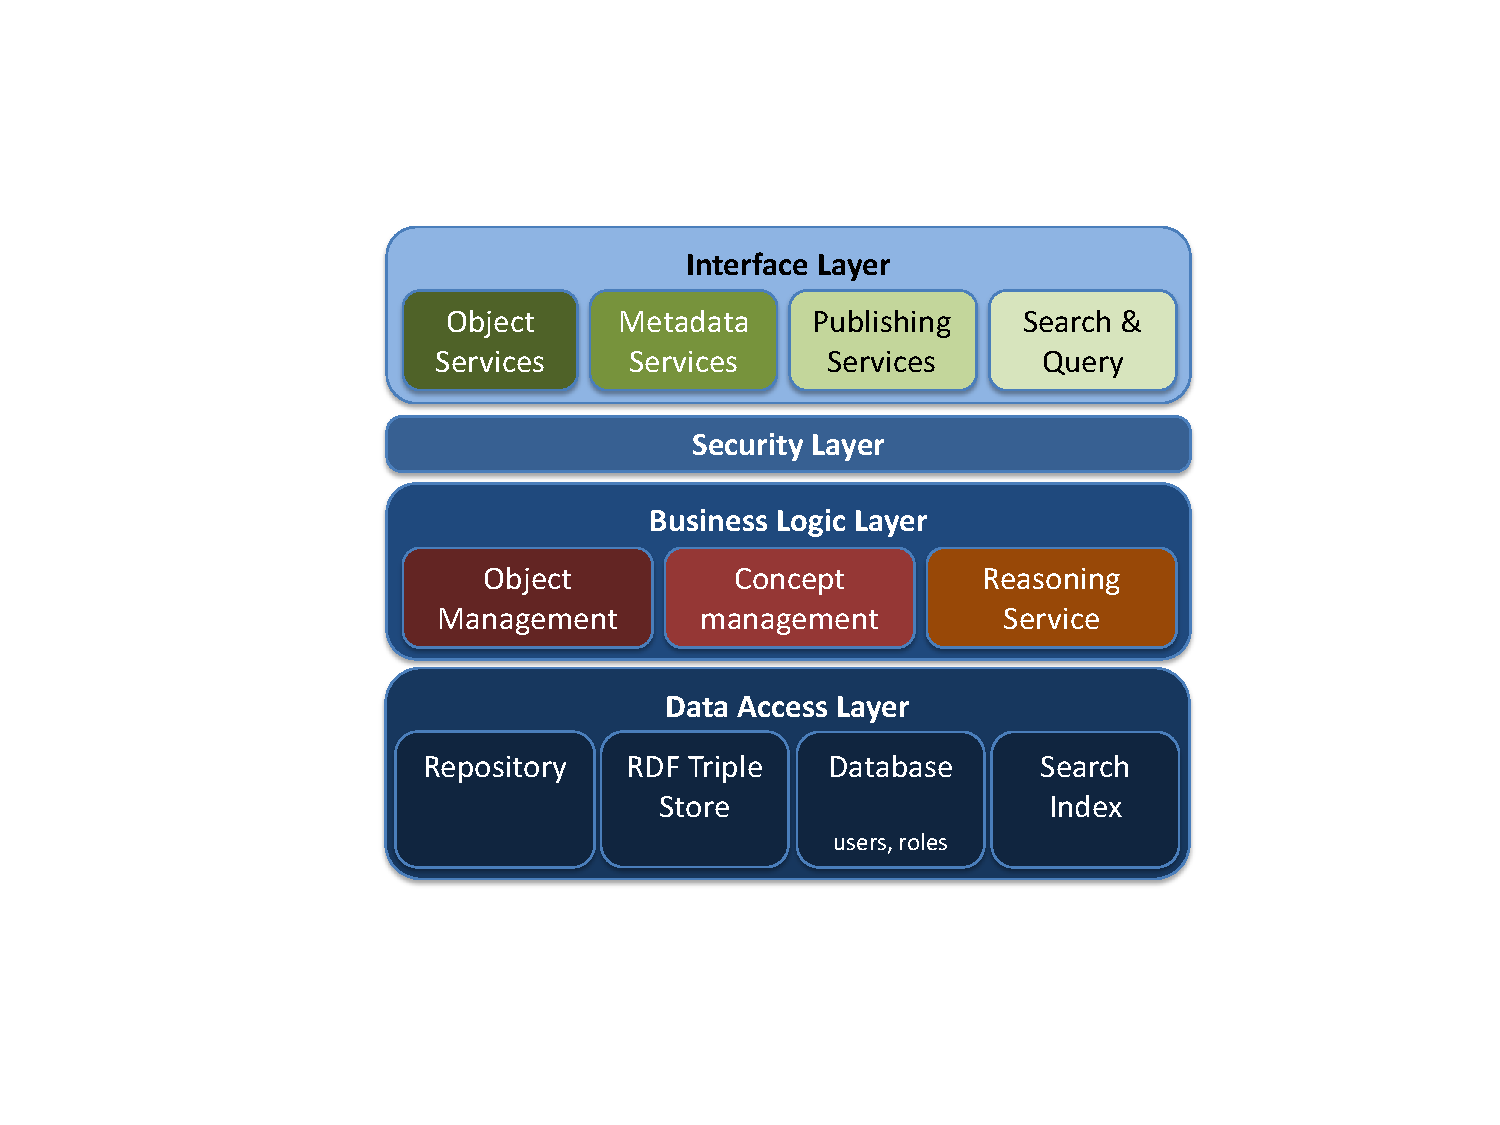
\includegraphics[trim = 60mm 30mm 50mm 36mm, clip,height=75mm]{architecture.pdf}
\vspace{-16pt} \caption{A high-level depiction of components in the ontology-driven
architecture.}\label{fig:arch}
\end{figure}

The high-level design of ontology-driven architecture takes a modular
and layered approach, as can be seen in Figure~\ref{fig:arch}.
At the foundation is the \textbf{data access layer},
consisting of an underlying repository system, an RDF triple store, an
in-house database that stores essential information and a full-text search
engine. This layer is responsible for low-level tasks when the creation,
modification and deletion of concepts and objects occur.
The \textbf{business logic layer} in the middle is responsible for
managing concepts and objects, such as versioning, object conversion
and integrity validation. The \textbf{security layer} controls access
(authentication and authorization) to concepts and objects and guards
all operations on them. In this architecture, authorization is based
on user attributes, which have two dimensions. Firstly, each user has
a system-wide role, such as registered user or system administrator, which
is used to determine access rights across the system.
Secondly, a project-wide role, such as project administrator and
project observer, can be assigned to a user so that he can have
project-specific access rights. At the top of the stack is
the \textbf{interface layer}, where the data management
system can be accessed using a number of interfaces such as a Web
browser or API calls.

%In this section, we presented the PODD conceptual and system
%architecture that can effectively support concept dynamics
%through an ontology-driven design. In the next section, we present
%details of the PODD domain ontology in a bioinformatics setting.

\section{Ontology-based Domain Modeling}\label{sec:ont}
%One of the important design decisions to be made early in the
%development process is the domain model. Domain modeling aims at
%providing solutions for two important tasks. Firstly, efficient and
%flexible data organization; and secondly, data contextualization in
%the form of \emph{metadata}, so as to provide meaning for the raw
%data (documents, publications, image files, etc.) to facilitate
%search, query, dissemination, and so on.

As we emphasized previously, the domain model should be flexible
enough to accommodate the rapid changes and dynamic nature of
scientific research. In this section, we present the base
ontology and the roles it plays in the ontology-driven
architecture. It should be noted that the architecture
proposed here is domain-independent and it be applied
to any scientific discipline that
shares a similar high-level domain model.

%Section~\ref{sec:podd_ont} describes the PODD ontology in detail,
%introducing essential domain concepts and the how inter-relationships
%and attributes are modeled. Section~\ref{sec:rav}
%describes the important roles the domain ontology performs at the
%various stages of object lifecycle.

\subsection{The Base Domain Ontology}\label{sec:podd_ont}
Inspired by FuGe and OBI, we create the base domain ontology
in OWL to define essential domain concepts, their attributes
and inter-relationships in an object-oriented fashion.
As stated in the previous section,
domain concepts will be modeled as OWL classes; relationships
between concepts and object attributes will be modeled as OWL object and
datatype properties. Concrete objects will be modeled as OWL
individuals.

For an overview, attributes and inter-relationships of some
of the domain concepts and the core metadata of all concepts
in this ontology are shown in Figure~\ref{fig:model}.

\begin{figure}[htb]
\centering
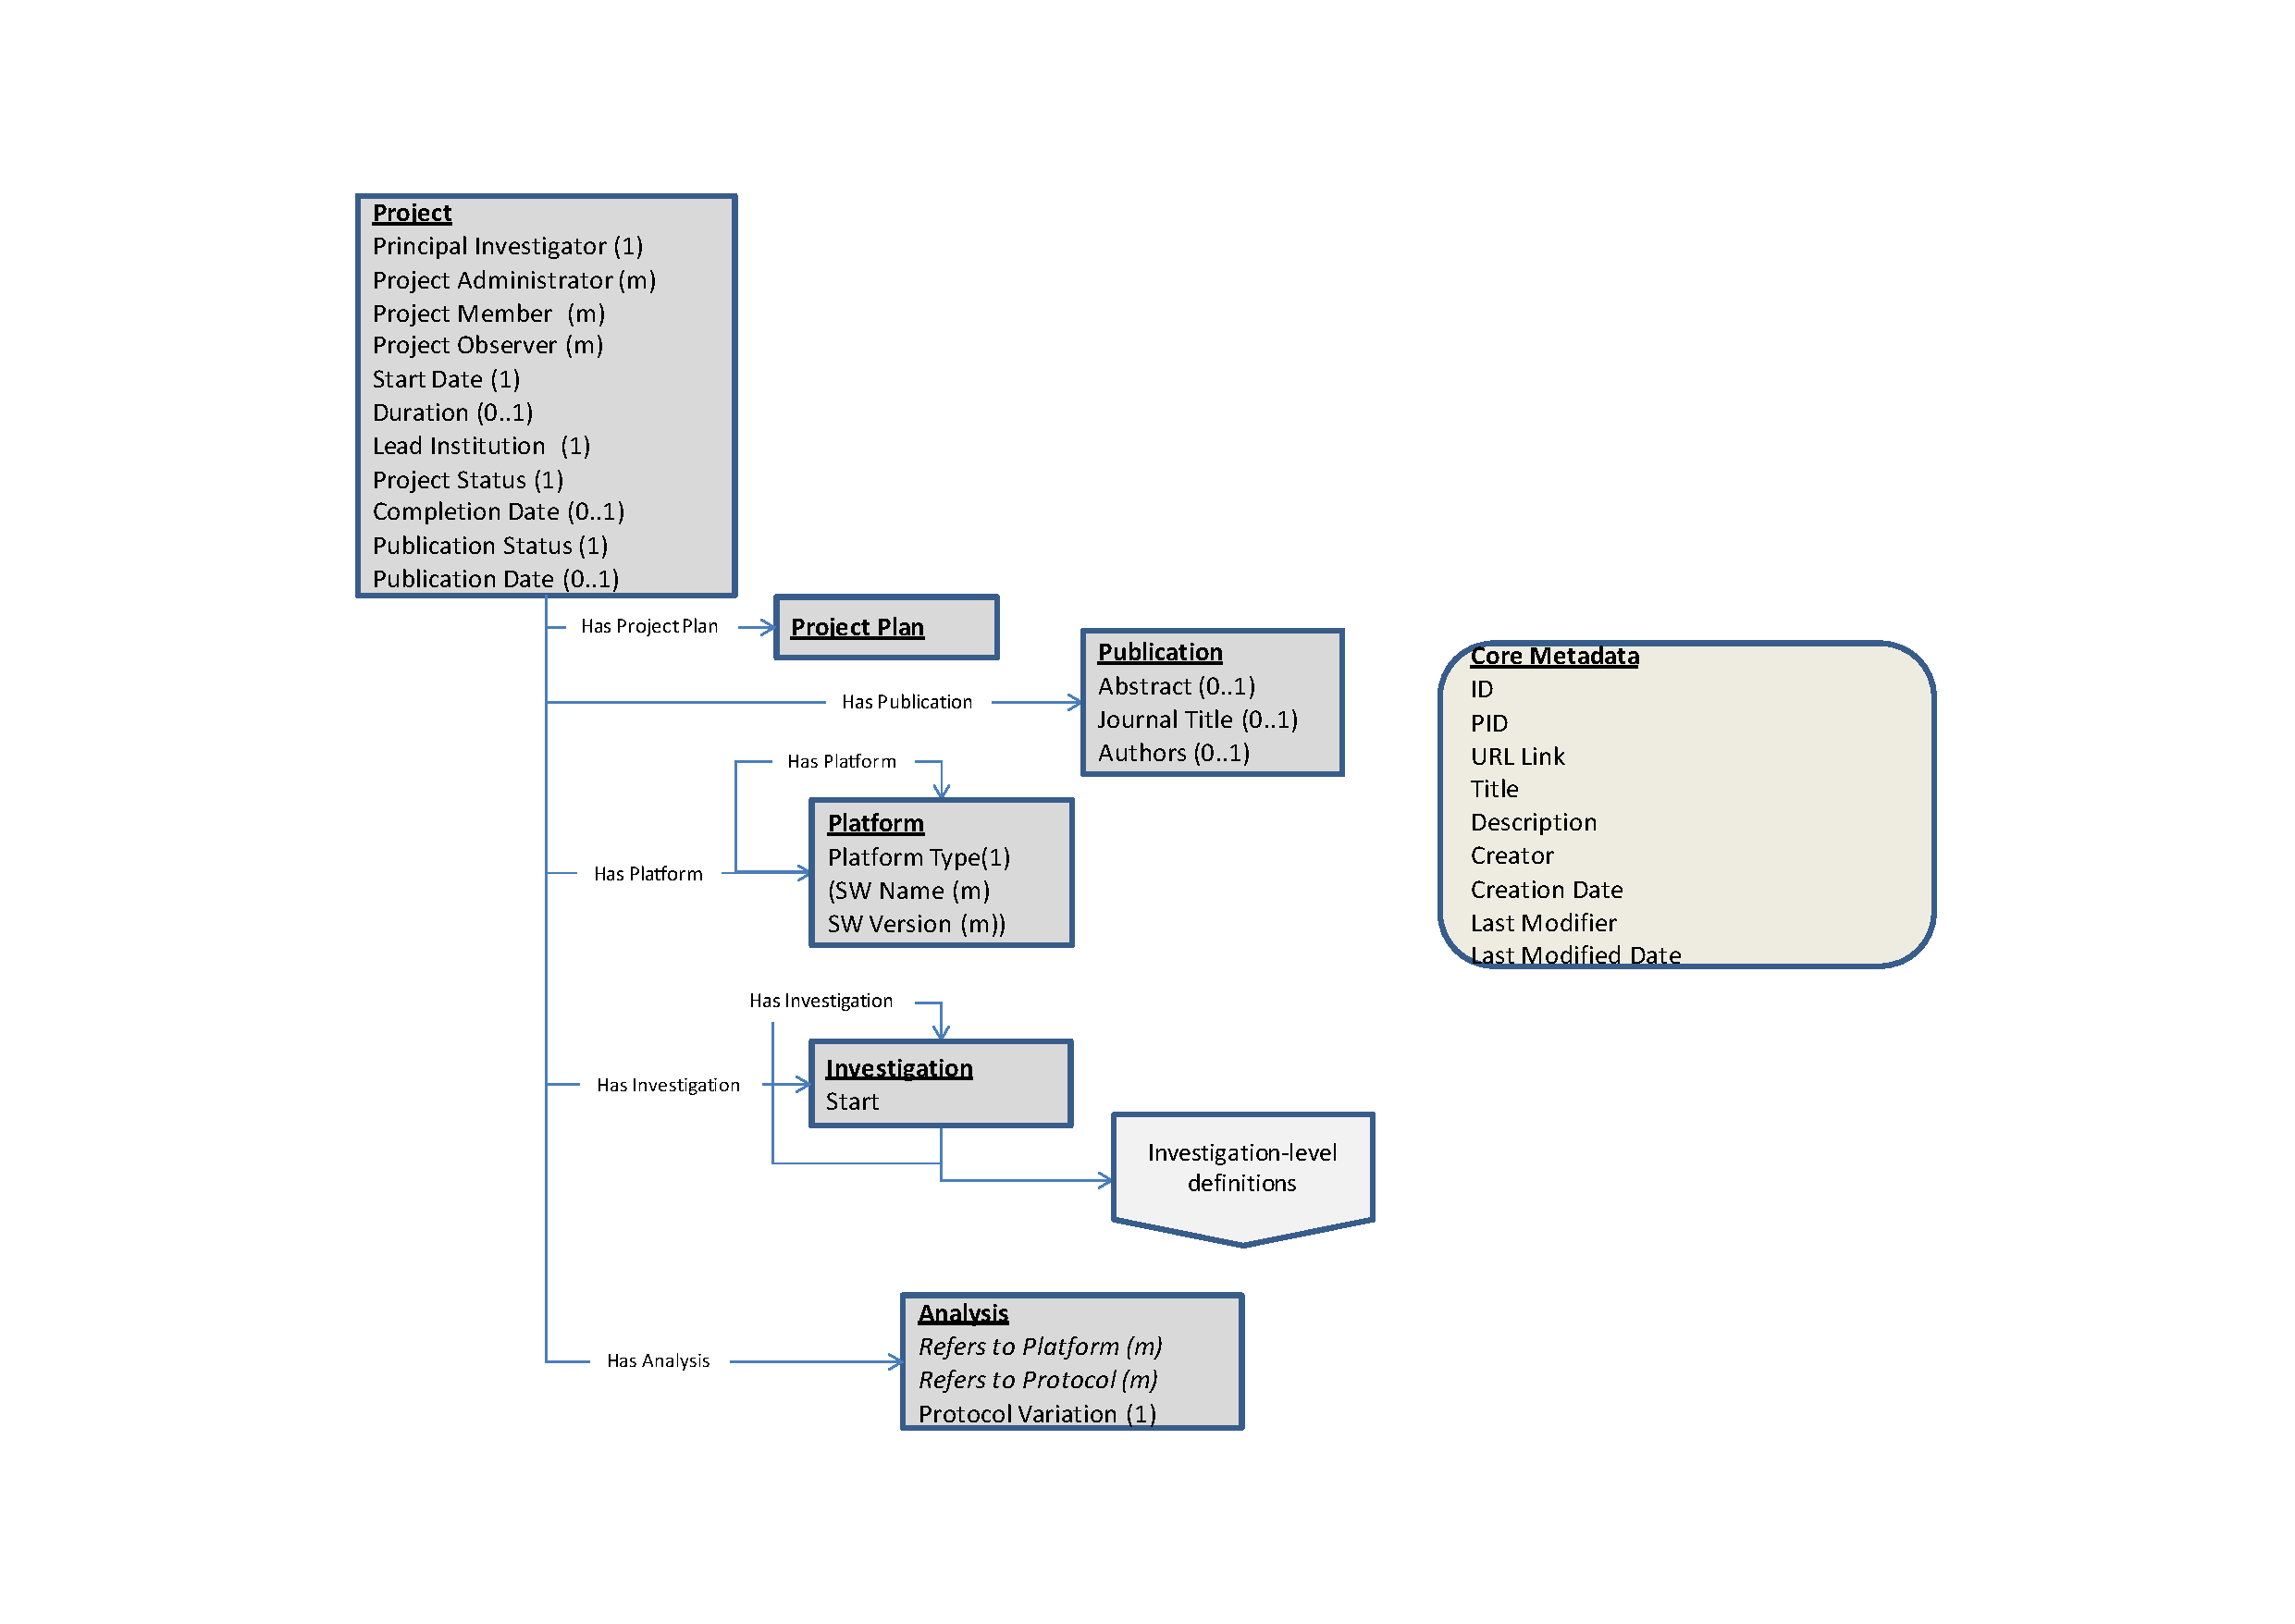
\includegraphics[trim = 54mm 20mm 64mm 30mm, clip,height=92mm]{model.pdf}
\vspace{-16pt} \caption{The attributes and relationships of some
domain concepts.}\label{fig:model}
\end{figure}

First of all, we set out a few design principles of
the domain ontology.
\begin{itemize}
\item All essential domain concepts are modeled as subclasses of
an abstract top-level OWL class \textbf{\emph{PODDConcept}} that
captures common attributes and relationships.

\item All relationships between domain concepts are captured by
\emph{domain properties}, which can be further divided into two
\emph{property hierarchies}, one for parent-child relationships
and the other for reference relationships. Each of the two
hierarchies have an abstract top-level property, called
\textbf{\emph{contains}} and \textbf{\emph{refersTo}}, respectively.

\item All parent-child relationships are
modeled in a property hierarchy as subproperties of the abstract
property \textbf{\emph{contains}}, and all reference relationships
are modeled in another property hierarchy as subproperties of the
abstract property \textbf{\emph{refersTo}}.

\item For each domain concept $T$, one property is defined in each
of the above hierarchies with its range defined to be $T$.
The domains of such properties are not specified so that
they can be used by any applicable domain concept to establish
a relationship between them.

\item Domain concepts (except \textbf{\emph{PODDConcept}})
are mutually disjoint with each other.

\item Essential domain concepts can be subclassed to provide more
specialized and refined information.
\end{itemize}

Moreover, to ensure that each object can have at most one parent object,
the inverse property of \textbf{\emph{contains}},
\textbf{\emph{isContainedBy}}, is defined so that a max cardinality
restriction can be added to the top-level concept \textbf{\emph{PODDConcept}}
to enforce it.

The definitions of the high-level constructs can be summarized
in Figure~\ref{fig:top}, in OWL DL syntax~\cite{hoph03a}.

\vspace{-8pt}
\begin{figure}[htb]
\small\centering
\begin{align*}
&PODDConcept \sqsubseteq \top & isContainedBy = (^-contains)\\
&\top \sqsubseteq \forall contains. PODDConcept
&\top \sqsubseteq \forall refersTo. PODDConcept\\
&PODDConcept \sqsubseteq \leq 1~ isContainedBy
\end{align*}

\vspace{-8pt}
\caption{Top-level ontology constructs in the PODD ontology.}\label{fig:top}
\end{figure}

\subsubsection{The Domain Concepts}
In the base domain ontology, essential domain classes include the following:

\begin{description}
\item[\emph{Project}] is the top-level
concept (under \textbf{\emph{PODDConcept}}) representing
an administrative concept that contains essential meta
information about the research project, such as the
administering organization, principal
investigator, project membership, project status, etc.

\item[\emph{ProjectPlan}] describing the research
plan of the project at the core metadata element level.

\item[\emph{Platform}] describing any single technical
measurement platform used in the project. Technical measurement
platform means any platform for which parameters and parameter
values may be captured.

%\item[\emph{Genotype}] describing the genotype of the
%materials used in the investigations. Multiple genotypes are
%described here and then can become fields in the instances of the
%Material object.

\item[\emph{Investigation}] describing a planned process
within a project that executes some form of study design and
produces a coherent set of results. It can be considered equivalent
to an experiment.

The \textbf{\emph{Investigation}} concept is of central importance.
It captures the data and metadata of experiments under a project. A
number of concepts are defined to assist in the modeling of
investigations.

\item[\emph{Design}] describing experimental design
components, e.g. plant layouts, sampling strategies, etc.

%\item[\emph{Growth Condition}] describing growth conditions, such as
%growth chambers used, environmental settings, etc.

\item[\emph{Process}] representing a planned component of an
investigation. It is a description of a series of steps taken to
achieve the objective of the investigation.

\item[\emph{Protocol}] describing a step within a process that is a
consistent whole. e.g. sterilize seeds, plant seedlings, image the
plants.

\item[\emph{Material}] describing the materials used in the
investigation. Materials can be either inputs or outputs. They can
be chemicals, substrates, whole organisms or samples taken from a
whole organism. The meaning of the \emph{Material} is usually
dependent on the domain and hence can be specified by domain-specific
properties.

\item[\emph{Event}] capturing ad-hoc events and actions that occur
against an individual material. In most instances the events and
their timing are described in the process/protocol. An \emph{Event} object
can be utilized to either record fixed events in a form that allows
for investigative analysis, or to record one off observations (e.g., the
plant under observation died).

\item[\emph{Measurement}] describing a single measurement against a
single material. e.g. an image of a plant is a single measurement.
\emph{Measurement} objects can capture measurement variables (e.g. shutter
speed, lighting, etc).

\item[\emph{Analysis}] is a metadata concepts used to describe
outputs derived from measurements. An analysis can be performed
against a single material object, a set of investigations,
or at the level of the whole project.
\end{description}

\subsubsection{Inter-concept Relationships}
The structures and workflows of phenomics research activities are
captured using OWL object properties.

%Different research projects will utilize different measurement
%platforms and have significantly different approaches and project
%designs. As a result, different projects may have different
%structures. In OWL, there are a number of ways of defining the same
%relationship. In order to achieve high modeling flexibility and
%accommodate as many scenarios as possible, we have made the
%following design decisions:

Following the design principles presented in the beginning of this
section, domain properties such as \textbf{\emph{hasAnalysis}}
and \textbf{\emph{refersToPlatform}} can be defined as follows
in Figure~\ref{fig:props}.

\vspace{-8pt}
\begin{figure}[htb]
\small\centering
\begin{align*}
&hasAnalysis\sqsubseteq contains & refersToPlatform \sqsubseteq refersTo\\
&\top\sqsubseteq \forall hasAnalysis.Analysis & \top \sqsubseteq \forall refersToPlatform.Platform
\end{align*}

\vspace{-8pt}
\caption{Example definitions of domain properties}\label{fig:props}
\end{figure}

%For each of the concepts described in the previous subsection except
%for \emph{Project}, we define an OWL object-predicate with the range
%being the concept. For example, for concept \emph{Analysis}, we
%define a predicate \emph{hasAnalysis} and define its range to be
%\emph{Analysis}.

\subsubsection{Object Attributes}
Attributes are intrinsic properties of an object, such as the status
of a project, the start date of an investigation and the timestamp
of an event. In our model, we use OWL properties to model object
attributes, similar to the modeling of inter-object relationships.

When the possible values of a particular attribute can be enumerated,
such as project status (\emph{active}, \emph{inactive} and \emph{completed}),
an enumerated OWL class is used to represent all the values.
When an attribute represents a grouping of some values, such
as accessions, where an accession has a source and a number,
an OWL class is also defined to represent the grouping.
In this case, auxiliary OWL properties are defined to project
out specific values in the grouping. In all other cases, attributes
are modeled using datatypes.

Figure~\ref{fig:project_owl} shows the partial definition of the OWL
class $Project$. Restriction
(\ref{for:hasPlan}), for example, states that any $Project$ instance must have
exactly one $ProjectPlan$ (through the predicate $hasProjectPlan$,
the range of which is $ProjectPlan$). The other 3 restrictions are
similarly defined.

\vspace{-8pt}
\begin{figure}[htb]
\centering
\small
\begin{align}
Project &\sqsubseteq~ =~ 1~ hasProjectPlan\label{for:hasPlan}\\
        &\sqsubseteq~ \geq~ 1~ hasInvestigation\\
        &\sqsubseteq~ =~ 1~ hasStartDate\\
        &\sqsubseteq~ \leq~ 1~ hasPublicationDate
\end{align}
\vspace{-16pt} \caption{Partial OWL Definition for the Project
concept.}\label{fig:project_owl}
\end{figure}

\subsection{Roles of Domain Ontologies in Object Life Cycle}\label{sec:rav}
The base ontology defines essential concepts independent of the domain.
Domain-specific information can be then captured by extending the
base ontology in individual systems.

Concrete objects which are instantiations of various concepts such as
\textbf{\emph{Project}} and \textbf{\emph{Investigation}}, are stored
in the repository and can
subsequently be retrieved for different purposes. As stated in
Section~\ref{sec:intro}, the ontology-based domain model is at the
center of the whole life cycle of objects. In this subsection, we
briefly describe the roles the domain ontologies perform at
various stages of the object life cycle.

\begin{description}
\item[Ingestion] When an object is created, the user specifies which
type of object she intends to create and the repository will pull up
all the ontological definitions for that type (from the OWL class
corresponding to that type and its super classes). Such definitions
will be used to (a) guide the rendering of object creation
interfaces and (b) validate the attributes and inter-object
relationships the user has entered before the object is ingested.
When the object is ingested, its metadata definitions are stored
as RDF assertions.

\item[Retrieval \& update] When an object is retrieved from the repository,
its attributes and inter-object relations are retrieved from its
RDF assertions, which are used to drive the on-screen rendering.
When any value is updated, it is validated and updated in this
object's RDF assertions.

\item[Query \& search] An object's assertions will be stored
in an RDF~\cite{rdfprimer04} triple store, which can be queried
using the SPARQL~\cite{sparql} query language. Similarly, ontology
definitions are indexed to provide functionalities such as full-text
search and faceted browsing.

\item[Publication \& export] When an object is published or exported,
its metadata, in RDF, will be retrieved and exported.
\end{description}

\subsection{Integration with Existing Domain Ontologies}
As stated before, ontologies such as Gene
Ontology~\cite{citeulike:212874} and Plant
Ontology~\cite{citeulike:3008167} are widely used in biomedical
research to capture information such as genes, proteins, sequences
and organism phenotypes. In our ontology-driven approach, these
ontologies will be used to add annotations on domain objects to
enrich their semantic descriptions and enable cross-application
reference and integration.

In summary, ontology-based domain modeling enables us to build very
expressive and extensible conceptual models which can be extended
to accommodate individual domains. Ample tool
support is also available to perform ontology-based tasks such as
validation, query answering and searching.
%In the next section,
%we describe our effort in building the PODD data management system
%based on the ontology-driven architecture and discuss in more detail
%the roles the ontology plays.

\section{The PODD Data Management System}\label{sec:podd}

Based on the ontology-driven architecture presented in Section~\ref{sec:design}
and the domain ontology presented in Section~\ref{sec:ont},
we have developed the PODD data management system to meet the
data management challenges faced by the Australian phenomics
research community.

To describe domain knowledge in phenomics, we extend the base
ontology described in Section~\ref{sec:ont} by defining the
following concepts: \emph{Genotype}, \emph{Gene}, \emph{Phenotype}
and \emph{Sequence} as subclasses of \emph{PODDConcept}. Additional
OWL object and datatype properties are also defined to model the
attributes and relationships of these concepts, such as shown in
Figure~\ref{fig:phe_ont}. Note that the last two definitions
integrate the new definitions with those in the base ontology.

\vspace{-8pt}
\begin{figure}[htb]
\small
\centering
\begin{minipage}[t]{.55\linewidth}
\centering
\begin{align*}
Genotype &\sqsubseteq~ PODDConcept\label{for:hasPlan}\\
         &\sqsubseteq~ \forall hasGene.Gene\\
         &\sqsubseteq~ \leq~ 1~ hasEcotype\\
         &\sqsubseteq~ \leq~ 1~ hasSubspecies\\
         &\cdots\\
Phenotype & \sqsubseteq PODDConcept\\
          & \sqsubseteq \forall hasMeasurement.Measurement\\
         &\cdots
\end{align*}
\end{minipage}
\begin{minipage}[t]{.4\linewidth}
\centering
\begin{align*}
Gene & \sqsubseteq~ PODDConcept\\
     & \sqsubseteq~ \forall hasSequence.Sequence\\
     & \sqsubseteq~ \leq~ 1~ hasAlias\\
     & \sqsubseteq~ \leq~ 1~ hasChromosome\\
     & \cdots
\end{align*}
\end{minipage}
\begin{align*}
Project & \sqsubseteq \forall hasGenotype.Genotype\\
Material & \sqsubseteq \forall hasPhenotype.Phenotype\\
         & \sqsubseteq \forall refersToGenotype.Genotype
\end{align*}

\vspace{-8pt}
\caption{Domain-specific OWL defintions.}\label{fig:phe_ont}
\end{figure}

The above definitions show how the new OWL classes are
integrated with existing ones through the use of OWL
object properties. Conceptually, it states that phenotype
objects are attached to material objects, which in turn
can reference genotype objects, which are defined as child
objects of projects.

As can be seen above, the domain model is dynamic in that
it accommodates the addition of new classes and properties.
As a result, the other components of the PODD system is also
designed to be amenable to the dynamic nature of the architecture.
%The Web interface is dynamically generated by reading the domain
%ontologies and translating the various ontological constructs
%(OWL restrictions, for example)
%into familiar Web elements. Such a principled approach
%makes the user interface layer both extensible and easy to use.
%
The PODD system is developed in Java for its cross-platform
availability and the huge ecosystem around it. A more detailed
architecture diagram for PODD can be seen in
Figure~\ref{fig:podd_arch}. Below we summarize a number of core
technologies employed in the development of the PODD data management
system and describe briefly how we use them to achieve extensibility
and scability.

\begin{figure}[htb]
\centering
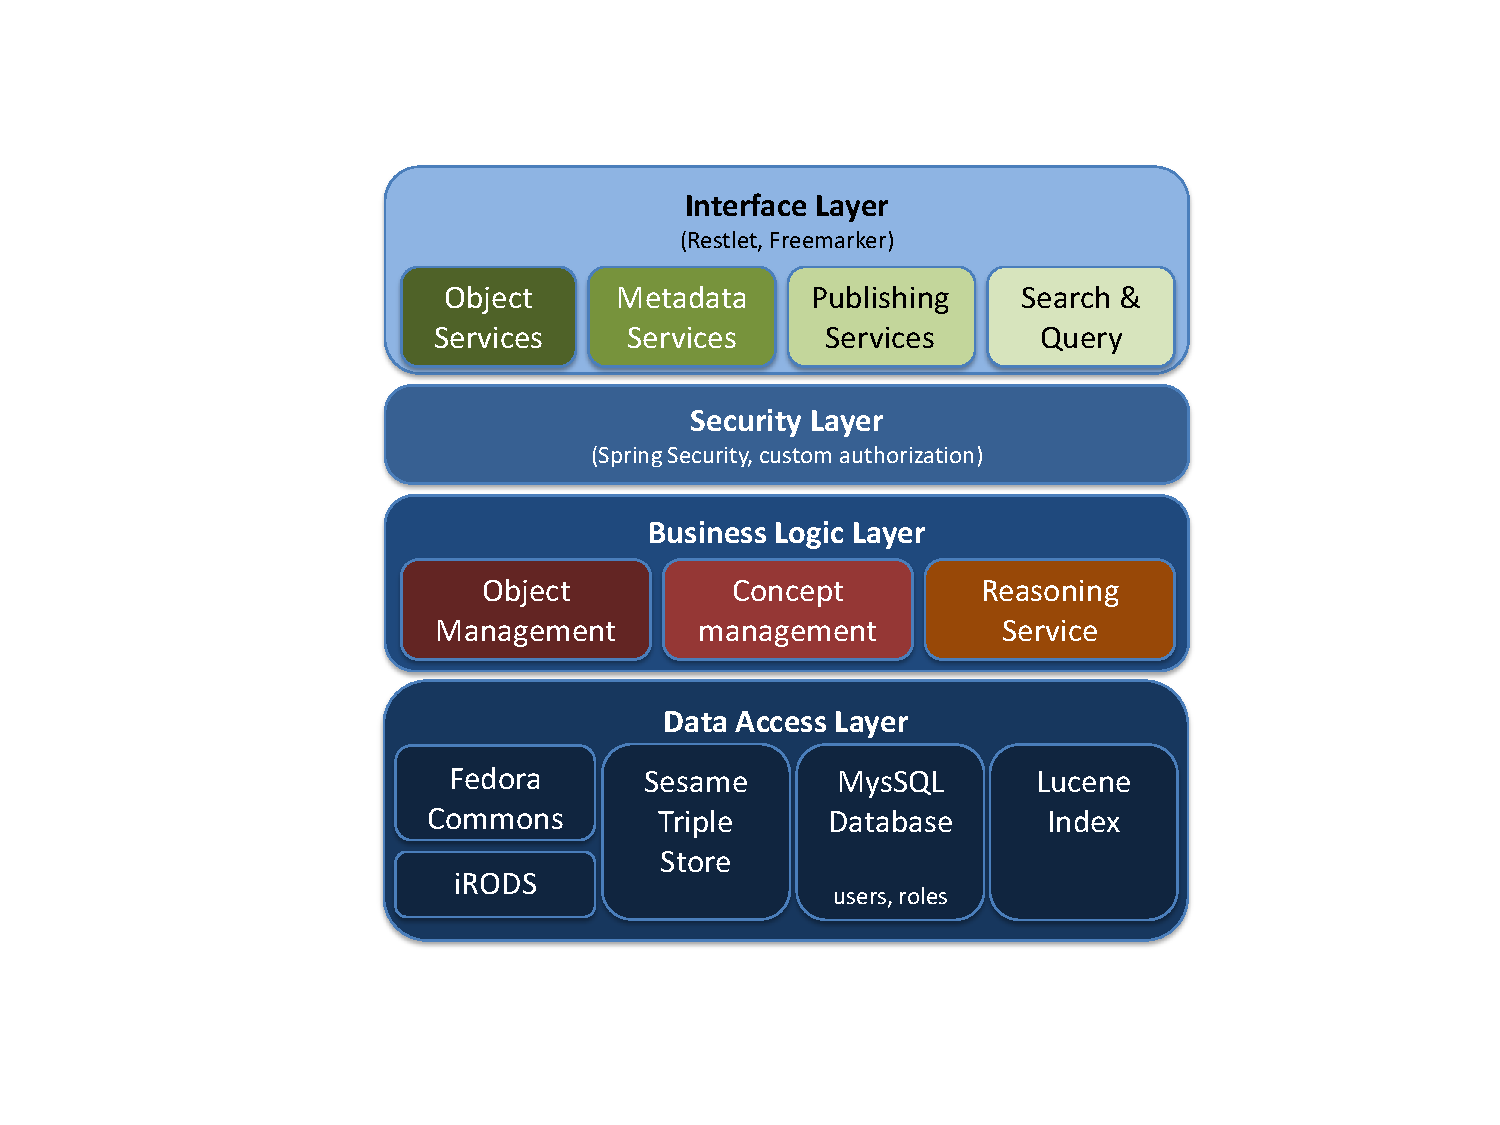
\includegraphics[trim = 60mm 30mm 50mm 28mm, clip,height=75mm]{podd_arch.pdf}
\vspace{-8pt} \caption{The architecture and components of
PODD.}\label{fig:podd_arch}
\end{figure}

\begin{itemize}
\item We use Fedora Commons, a digital repository for the
storage and retrieval of domain objects.

As introduced in Section~\ref{sec:overview}, Fedora Commons is a mature,
widely-used digital repository software. In PODD, we store domain concepts as
Fedora models and concrete domain objects as Fedora objects. The OWL (for
concepts) and RDF (for objects) definition of each concept and object
is stored in a special versioned datastream \texttt{PODD}, which is used
by the system in various tasks such as object creation, rendering, validation
and update. Moreover, raw data files are also stored in Fedora Commons
as versioned datastreams.

It is to be noted that the structure of domain objects is not maintained
in Fedora Commons but rather in PODD system on top of it. In other words,
Fedora Commons is not aware of the semantics of concepts and objects.

\item We use iRODS~\cite{irods07}, a distributed, grid-based storage
software system, as the storage module for Fedora Commons to provide
a distributed storage solution. Transparent to Fedora Commons,
iRODS manages the distribution and replication across a virtual,
geographically-distributed data fabric.

iRODS provides two important
benefits: (1) data transfer can enjoy principle of locality by
replicating files at strategically placed data storage nodes in the fabric;
and (2) storage size is theoretically unlimited as the data fabric can
grow as demand grows.

\item We incorporate the Sesame\footnote{\url{http://www.openrdf.org/}}
triple store to support complex query answering with SPARQL. It also
provides metadata to the full-text index and search component.

For each object, its RDF definitions are stored in a
Sesame \emph{context} that uniquely scopes and identifies
the triples. The use of contexts is necessitated by
two facts. Firstly, it cannot be guaranteed that triples are
unique across all objects. For example, \emph{Accession}
objects are defined as RDF blank nodes with an accession
source and an accession number. Hence, it is possible
that two objects contain the \emph{same} accession object,
which cannot be distinguished in the triple store. Hence,
contexts are necessary to identify all triples of a given
object. Secondly, as described in Section~\ref{sec:design},
access control needs to be enforced on a project level.
Similarly, it also needs to be enforced on query answering
in the triple store. By identifying triples of individual
objects, we are able to control contexts a user can access
through query expansion.

\item We use the Solr\footnote{\url{http://lucene.apache.org/solr/}}
open-source search engine platform to provide full-text search
and faceted browsing capabilities of repository
contents, including values in the RDF triple store.

Similar to the structure of the Sesame triple store,
there is a one-to-one correspondence between domain objects
in the repository and the Solr \emph{documents}, which
represent logical indexing units. Moreover, through
search query expansion, access control can be applied to
search results.

\item We use MySQL database to store user and access control
related information, as it is orthogonal to other domain
concepts.

\end{itemize}

Figure~\ref{fig:browser} shows the browser view of a plant phenomics
project that investigates Arabidopsis. Note that in this view, the
objects are shown in a tree-like structure by following the property
assertions of subproperties of \emph{contains} defined in the base
and domain ontologies.

\begin{figure}[htb]
\centering
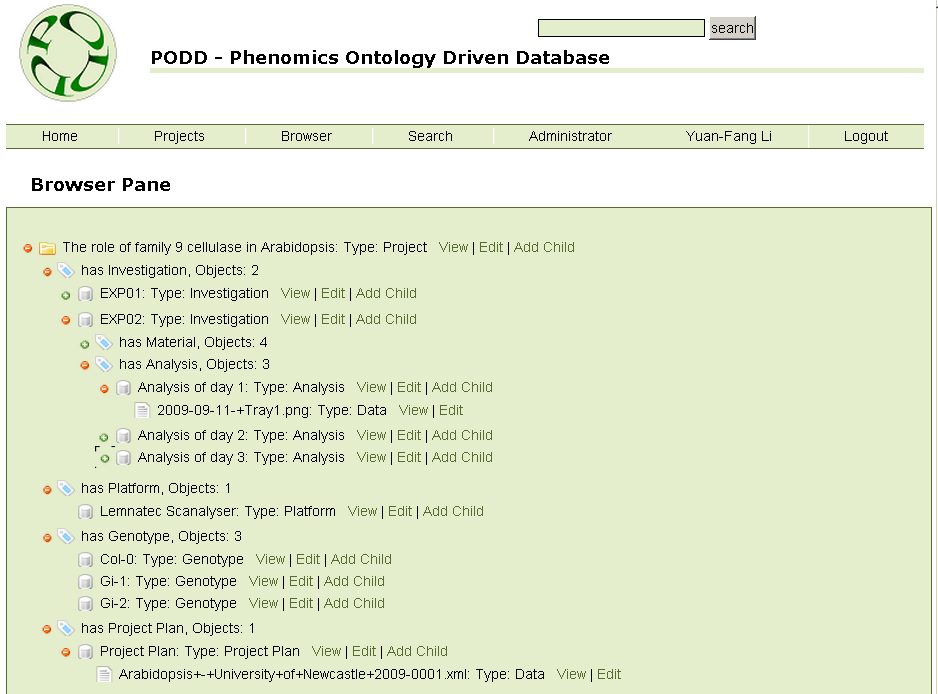
\includegraphics[trim = 0mm 2mm 5mm 0mm, clip,width=120mm]{browser.png}
\vspace{-4pt} \caption{The browser view of a plant phenomics project
in PODD.}\label{fig:browser}
\end{figure}

Following the ontology-driven architecture and through the use
of mature technologies, we have successfully developed PODD, a
scalable, extensible data management system. At the same time,
data management tasks such as versioning, logical organization
of data, authentication \& authorization, and discovery, can
all be supported effectively. In summary, the PODD system
demonstrates the feasibility and practicality of the proposed
ontology-driven architecture.

\section{Conclusion}\label{sec:conclusion}
Sound data management practice is a challenge faced by
many data-intensive scientific disciplines. A number of
root causes contribute to this challenge.
Firstly, scientific advancement
usually connotes that the conceptual data model is being
continually evolved, requiring the data management system
to be sufficiently adaptive to accommodate future changes.
Secondly, huge amounts of data are being generated off a
wide variety of instruments and software, requiring the data
management system to be highly scalable for efficient data
processing. Moreover, an important requirement of data management
systems is to organize data in a logical way to facilitate
tasks such as curation, integration, discovery and dissemination.
Hence, the management of metadata is of central importance.

Traditional data management systems are typically developed
around a relational database in which database schemas
define the domain model and constraints on
abstract concepts. A change in schema design normally
requires database migration, which is an error-prone
process. As a result, such systems are not best
suited in a dynamic environment where model evolution is
the norm rather than the exception.

In recent years a number of repository systems such as
Fedora Commons and Apache Jackrabbit have been developed.
These systems impose minimal modeling constraints and hence
are more flexible. As a consequence, however, rich logical
structures of data cannot be easily expressed and maintained
in such systems.

Given their intrinsic characteristics of semantic rigor and
open nature, we believe ontology languages such as OWL and
RDFS are an ideal conceptual foundation on which effective
data management systems can be built. In this paper, we
propose an ontology-driven architecture for developing data
management systems that are able to handle dynamic data and models.

In our architecture, an ontology defines the behaviors of and
relationships between domain objects using OWL vocabularies. Such
definitions play a central role in all data management tasks
including data acquisition, validation, presentation, discovery and
integration.

We present the base ontology which encodes essential domain
knowledge to describe the structure of the data through the use of
OWL restrictions. The base ontology is designed in a way to strike a
balance between richness in modeling capabilities and the ease of
realization of data management requirements such as flexible
authentication and authorization. Moreover, the base ontology can be
naturally specialized to provide domain-specific definitions to
cater for the different needs of individual disciplines.

Phenomics is an emergent research discipline that is poised to have
a significant impact upon industrial-scale biological research.
Phenomics presents a number of data management challenges, such as
the management of evolving technologies and large volumes of data
and the integration of highly heterogeneous datasets. Consequently
phenomics represents an ideal domain for illustrating our
ontology-driven approach to research data management.

To validate the feasibility of the ontology-driven architecture
and to meet the data management needs of the Australian phenomics
research community, we developed the PODD repository to enable
efficient storage, retrieval, contextualization, query, discovery
and publication of large amounts of data.

Through the employment of the ontology-driven architecture,
the domain ontology and underlying repository system (Fedora
Commons), the PODD repository is highly adaptive that
the addition of new concepts and the modification
of existing concepts do not affect data already present
in the system. It is also able to perform effective data
management tasks over a large and growing amount of data.

In summary, our contribution in this work is three-fold: firstly,
the proposal of the ontology-driven architecture for developing data
management systems; secondly, the development of a base ontology
that defines essential domain knowledge; and thirdly, the
development of the PODD data management system in the validation of
the practicality of the proposed approach. To the best of our
knowledge, this is the first proposal of an ontology-driven
architecture for scientific data management systems.

We have identified a number of future work directions that
we would like to pursue. Firstly, we will investigate into the
integration with existing domain ontologies such as the
Gene Ontology~\cite{citeulike:212874} and the Plant
Ontology~\cite{citeulike:3008167}. One possibility
would be to use terms defined in these ontologies to
annotate metadata objects~\cite{1419711}. Secondly, we would like to
investigate the generalization of the ontology-driven
approach so that it can be applied to other areas such
as workflow management systems.
Thirdly, we will continue the development of the PODD system
to provide additional functionalities such as
data visualization, automated data integration and
Linked Data-style data discovery and publication.

\section*{Acknowledgement}
The authors wish to acknowledge the support of the National
eResearch Architecture Taskforce (NeAT) and the Integrated
Biological Sciences Steering Committee (IBSSC) Australia. The authors wish to
thank Dr Xavier Sirault, Dr. Kai Xu and Mr. Philip Wu for
the discussion on the development of the domain ontology
and the PODD system.

\bibliographystyle{elsarticle-num}
\newcommand{\gobble}[1]{}
\begin{thebibliography}{10}
\expandafter\ifx\csname url\endcsname\relax
  \def\url#1{\texttt{#1}}\fi
\expandafter\ifx\csname urlprefix\endcsname\relax\def\urlprefix{URL
}\fi \expandafter\ifx\csname href\endcsname\relax
  \def\href#1#2{#2} \def\path#1{#1}\fi

\bibitem{1107503}
J.~Gray, D.~T. Liu, M.~Nieto-Santisteban, A.~Szalay, D.~J. DeWitt,
G.~Heber,
  Scientific data management in the coming decade, SIGMOD Rec. 34~(4) (2005)
  34--41.
\newblock \href {http://dx.doi.org/http://doi.acm.org/10.1145/1107499.1107503}
  {\path{doi:http://doi.acm.org/10.1145/1107499.1107503}}.

\bibitem{brm2007}
A.~Shah, M.~Singhal, K.~Klicker, E.~Stephan, H.~Wiley, K.~Waters,
Enabling
  high-throughput data management for systems biology: The bioinformatics
  resource manager, Bioinformatics 23~(7) (2007) 906--909.

\bibitem{rdfschema04}
{D. Brickley and R.V. Guha (editors)}, {Resource Description
Framework (RDF)
  Schema Specification 1.0}, \url {http://www.w3.org/TR/rdf-schema/} (Feb.
  2004).

\bibitem{hoph03a}
I.~Horrocks, P.~F. Patel-Schneider, F.~van Harmelen, {From
$\mathcal{SHIQ}$ and
  {RDF} to {OWL}: The Making of a Web Ontology Language}, Journal of Web
  Semantics 1~(1) (2003) 7--26.

\bibitem{linkeddata}
T.~Berners-Lee, {Linked Data},
  \url{http://www.w3.org/DesignIssues/LinkedData.html} (2007).

\bibitem{aue07dbpedia}
S.~Auer, C.~Bizer, G.~Kobilarov, J.~Lehmann, R.~Cyganiak, Z.~Ives,
  \href{http://dx.doi.org/10.1007/978-3-540-76298-0_52}{{DBpedia: A Nucleus for
  a Web of Open Data}}, in: Proceedings of 6th International Semantic Web
  Conference, 2nd Asian Semantic Web Conference (ISWC+ASWC 2007), 2008, pp.
  722--735.
\newline\urlprefix\url{http://dx.doi.org/10.1007/978-3-540-76298-0_52}

\bibitem{journals/bib/RuttenbergRSM09}
A.~Ruttenberg, J.~Rees, M.~Samwald, M.~S. Marshall, {Life Sciences
on the
  Semantic Web: the Neurocommons and Beyond}, Briefings in Bioinformatics
  10~(2) (2009) 193--204.
\newblock \href {http://dx.doi.org/10.1093/bib/bbp004}
  {\path{doi:10.1093/bib/bbp004}}.

\bibitem{citeulike:1882392}
B.~Smith, M.~Ashburner, C.~Rosse, et~al., {The OBO Foundry:
Coordinated
  Evolution of Ontologies to Support Biomedical Data Integration}, Nature
  Biotechnology 25~(11) (2007) 1251--1255.
\newblock \href {http://dx.doi.org/10.1038/nbt1346}
  {\path{doi:10.1038/nbt1346}}.

\bibitem{citeulike:212874}
M.~Ashburner, C.~A. Ball, J.~A. Blake, et~al.,
  \href{http://dx.doi.org/10.1038/75556}{{Gene Ontology: Tool for the
  Unification of Biology}}, Nat Genet 25~(1) (2000) 25--29.
\newblock \href {http://dx.doi.org/10.1038/75556} {\path{doi:10.1038/75556}}.
\newline\urlprefix\url{http://dx.doi.org/10.1038/75556}

\bibitem{citeulike:5008761}
C.~Bizer, T.~Heath, T.~Berners-Lee, Linked data - the story so far,
  International Journal on Semantic Web and Information Systems (IJSWIS) 5~(3)
  (2009) 1--22.

\bibitem{podd_icadl}
Y.-F. Li, G.~Kennedy, F.~Davies, J.~Hunter, {PODD: An
Ontology-driven Data
  Repository for Collaborative Phenomics Research}, in: Proceedings of 12th
  International Conference on Asian Digital Libraries (ICADL 2010),
  Springer-Verlag, 2010, to appear.

\bibitem{dhoule09}
D.~Houle, {Numbering the Hairs on Our Heads: The Shared Challenge
and Promise
  of Phenomics}, {Proceedings of the National Academy of Sciences} 107 (2009)
  1793--1799.

\bibitem{Sauer200458}
U.~Sauer, {High-throughput Phenomics: Experimental Methods for
Mapping
  Fluxomes}, Current Opinion in Biotechnology 15~(1) (2004) 58--63.
\newblock \href
  {http://dx.doi.org/http://dx.doi.org/10.1016/j.copbio.2003.11.001}
  {\path{doi:http://dx.doi.org/10.1016/j.copbio.2003.11.001}}.

\bibitem{nevo01}
E.~Nevo, Evolution of genome-phenome diversity under environmental
stress,
  {Proceedings of the National Academy of Sciences} 98~(11) (2001) 6233--6240.

\bibitem{plant_furbank}
R.~T. Furbank, Plant phenomics: from gene to form and function,
Functional
  Plant Biology 36~(10) (2009) 5--6.

\bibitem{DBLP:journals/nar/WheelerBBBCCCDEFGHKKKLMMOPSSSSSSSSTTWY06}
D.~L. Wheeler, et~al., Database resources of the national center for
  biotechnology information, Nucleic Acids Research 34~(Database-Issue) (2006)
  173--180.

\bibitem{AmosBairoch01012005}
A.~Bairoch, et~al., {The Universal Protein Resource (UniProt)},
Nucl. Acids
  Res. 33~(suppl\_1) (2005) D154--159.
\newblock \href {http://dx.doi.org/10.1093/nar/gki070}
  {\path{doi:10.1093/nar/gki070}}.

\bibitem{783165}
C.~Baru, R.~Moore, A.~Rajasekar, M.~Wan, {The SDSC storage resource
broker},
  in: CASCON '98: Proceedings of the 1998 conference of the Centre for Advanced
  Studies on Collaborative research, IBM Press, 1998, p.~5.

\bibitem{652836}
W.~Hoschek, F.~J. Ja\'{e}n-Mart\'{\i}nez, A.~Samar, H.~Stockinger,
  K.~Stockinger, Data management in an international data grid project, in:
  GRID '00: Proceedings of the First IEEE/ACM International Workshop on Grid
  Computing, Springer-Verlag, London, UK, 2000, pp. 77--90.

\bibitem{565296}
K.~Krauter, R.~Buyya, M.~Maheswaran, A taxonomy and survey of grid
resource
  management systems for distributed computing, Softw. Pract. Exper. 32~(2)
  (2002) 135--164.
\newblock \href {http://dx.doi.org/http://dx.doi.org/10.1002/spe.432}
  {\path{doi:http://dx.doi.org/10.1002/spe.432}}.

\bibitem{Spallation_metadatamodel}
S.~Sufi, B.~Mathews,
\href{http://epubs.cclrc.ac.uk/bitstream/485/}{{CCLRC
  Scientific Metadata Model: Version 2}} (2004).
\newline\urlprefix\url{http://epubs.cclrc.ac.uk/bitstream/485/}

\bibitem{citeulike:3735746}
L.~N. Soldatova, R.~D. King,
\href{http://dx.doi.org/10.1098/rsif.2006.0134}{An
  ontology of scientific experiments.}, Journal of the Royal Society, Interface
  3~(11) (2006) 795--803.
\newblock \href {http://dx.doi.org/10.1098/rsif.2006.0134}
  {\path{doi:10.1098/rsif.2006.0134}}.
\newline\urlprefix\url{http://dx.doi.org/10.1098/rsif.2006.0134}

\bibitem{citeulike:151946}
A.~Brazma, et~al.,
\href{http://dx.doi.org/10.1038/ng1201-365}{{Minimum
  information about a microarray experiment (MIAME) -- toward standards for
  microarray data}}, Nat Genet 29~(4) (2001) 365--371.
\newblock \href {http://dx.doi.org/10.1038/ng1201-365}
  {\path{doi:10.1038/ng1201-365}}.
\newline\urlprefix\url{http://dx.doi.org/10.1038/ng1201-365}

\bibitem{citeulike:1756058}
A.~R. Jones, M.~Miller, R.~Aebersold, et~al., {The Functional
Genomics
  Experiment model (FuGE): an Extensible Framework for Standards in Functional
  Genomics}, Nature Biotechnology 25~(10) (2007) 1127--1133.
\newblock \href {http://dx.doi.org/10.1038/nbt1347}
  {\path{doi:10.1038/nbt1347}}.

\bibitem{rdfprimer04}
F.~Manola, E.~M. (editors), {{RDF Primer}},
  \url{http://www.w3.org/TR/rdf-primer/} (Feb. 2004).

\bibitem{sparql}
E.~Prud'hommeaux, A.~Seaborne, {SPARQL Query Language for RDF},
  \url{http://www.w3.org/TR/2006/CR-rdf-sparql-query-20060406/} (Apr. 2006).

\bibitem{irods07}
A.~Rajasekar, R.~Moore, F.~Vernon, {iRODS: A Distributed Data
Management
  Cyberinfrastructure for Observatories}, in: American Geophysical Union, Fall
  Meeting 2007, 2007.

\bibitem{citeulike:3008167}
S.~Avraham, C.-W. Tung, K.~Ilic, P.~Jaiswal, E.~A. Kellogg,
S.~Mccouch,
  A.~Pujar, L.~Reiser, S.~Y. Rhee, M.~M. Sachs, M.~Schaeffer, L.~Stein,
  P.~Stevens, L.~Vincent, F.~Zapata, D.~Ware,
  \href{http://dx.doi.org/10.1093/nar/gkm908}{The plant ontology database: a
  community resource for plant structure and developmental stages controlled
  vocabulary and annotations}, Nucl. Acids Res. 36~(suppl\_1) (2008) D449--454.
\newblock \href {http://dx.doi.org/10.1093/nar/gkm908}
  {\path{doi:10.1093/nar/gkm908}}.
\newline\urlprefix\url{http://dx.doi.org/10.1093/nar/gkm908}

\bibitem{1419711}
R.~Schroeter, J.~Hunter, A.~Newman, Annotating relationships between
multiple
  mixed-media digital objects by extending annotea, in: ESWC '07: Proceedings
  of the 4th European conference on The Semantic Web, Springer-Verlag, Berlin,
  Heidelberg, 2007, pp. 533--548.
\newblock \href
  {http://dx.doi.org/http://dx.doi.org/10.1007/978-3-540-72667-8\_38}
  {\path{doi:http://dx.doi.org/10.1007/978-3-540-72667-8\_38}}.

\end{thebibliography}

\end{document}
